\chapter{Implementation}
\label{chapter:implementation}
This chapter will provide insight on how the new user interface is implemented. First, a description of the frameworks and tools used is given in section~\ref{section:frameworkandtools}. Then, section~\ref{section:functionality} will give a brief description of the core components that drive the new user interface.

\section{Frameworks and tools}
\label{section:frameworkandtools}
The new user interface will be browser-based and is built with several modern frameworks and tools. Due to the highly adoptable characteristic of speech feedback, we have opted to use the Web Speech API, a W3C specification that is currently in development. At the time of writing, Google's Chrome browser offers the best support for this feature, and thus our new user interface requires the use of Chrome. More details on the Web Speech API are provided in section~\ref{subsection:webspeechapi}.

\subsection{REST API}
\label{subsection:restapi}
One of Apache Isis' core features is the availability of a \textit{\acrlong{rest}} (\acrshort{rest}) API. A \acrshort{rest} API provides a simple way of opening up an application to third party software or implementations. Unlike SOAP which uses remote objects, action invocations and encapsulated functionality, \acrshort{rest} only exposes data structures and their current state\cite{battle2008bridging}. It utilises HTTP to transfer its data and represents its data in JSON format, making it highly compatible with other technologies.

Richard Pawson, who conceived the \acrshort{no} \todo{zeg je dit voor het eerst? Dan uitschrijven!, een referentie is hier ook wel gepast} pattern, and Dan Haywood, lead committer of Apache Isis, have drafted the Restful Objects specification. This is an extension of the \acrshort{rest} specification with a set of rules to describe a domain model implementing the \acrshort{no} pattern\cite{Restf62:online}. Apache Isis implements the Restful Objects specification.

The \acrshort{rest} API allows us to easily connect our user interface to the existing back-end of any application. Once the user is authorised, only those services and objects that would be visible to the user in the standard user interface are exposed in the \acrshort{rest} API. Furthermore, the standardised technologies used in the API enables the use of a wide range of web frameworks, and thus we can pick one that caters best towards achieving the effective and simple interaction part of research question~\ref{RQ2}.

\subsection{AngularJS}
\label{subsection:angularjs}
One of the main areas of concern in our new user interface is that the target user group should not have to worry about anything that can impede the use of the application. Therefore, we have opted for AngularJS\cite{Angul50:online} as the framework to develop the new user interface in. AngularJS greatly simplifies the development of single-page applications, which is a valuable asset for our user interface. All user input is provided through one input field, and it is desirable that the user is unable to accidentally bring the input field out of focus. With a single-page application, the browser will never refresh, providing an uninterrupted user experience.

Furthermore, AngularJS has built-in support for consuming a \acrshort{rest} API through its \newline \texttt{\$resource} factory, reducing the complexity of the code needed to interact with the back-end of the application.

AngularJS distinguishes three main components:

\begin{itemize}
	\item The \textbf{scope} acts as the model in the framework, containing the data that is relevant to a certain state of the application.
	\item The \textbf{controller} processes user input and updates the scope with new values.
	\item The \textbf{view} is a dynamic representation of the scope data. If the controller updates the scope, the view will automatically represent the changes.
\end{itemize}

\subsection{Web Speech API}
\label{subsection:webspeechapi}
The Web Speech API is an interorganisational effort to make the internet more accessible through recognition and synthesis of speech\cite{WebSp68:online}. While it is currently still in development, Google Chrome offers full support of the specified functionality. After some initial experiments, we have concluded that the API's speech synthesis works remarkably well and is easy to use. Moreover, it works with JavaScript out-of-the-box and thus is easily integrable with the AngularJS application.

Aside from the speech synthesis functionality, the Web Speech API also offers speech recognition. Brief testing found that while the speech recognition functionality performed far better than expected, there were some issues to overcome when synthesis and recognition were combined which would be too time consuming to solve within the time frame of this research. If development continues after completion of this research it will definitely be implemented at some point, but for now we will adhere to keyboard input.

\section{Functionality}
\label{section:functionality}
This section will describe the AngularJS components that have been implemented. We will not cover the views, as they are simple HTML files that do not contain any significant functionality.

\subsection{Main module}
\label{subsection:mainmodule}
The main module \bfttt{app.js} is the core of the application. Its main task is to implement the routing between the different states in the application. We have used the UI-router addon\cite{angul39:online}, as it provides a lot of additional functionality over the default routing provided by AngularJS's \texttt{\$routeProvider}. 

At any time, the application has two active views, as shown in figure~\ref{figure:clisisviews}: the user input view and system output view. This is achieved by adding an abstract state \texttt{base}. While an abstract state can not be active itself, child states inherit all features that are assigned to the abstract state. In our case, \texttt{base} only defines the parent view, which divides the screen in two separate views. The user input view never changes, while the system output view is updated conforming to user input. The following states are defined:

\begin{itemize}
	\item \texttt{base.noOutput} displays a welcome screen.
	\item \texttt{base.home} displays the available menus.
	\item \texttt{base.services} displays the actions of a menu.
	\item \texttt{base.serviceAction} processes a menu action invocation. As this is an internal process, it has no view attached to it.
	\item \texttt{base.serviceActionParams} dispays parameters if a menu action requires them.
	\item \texttt{base.object} displays the properties, collections and actions of an object.
	\item \texttt{base.objectAction} processes an object action invocation. As this is an internal process, it has no view attached to it.
	\item \texttt{base.objectActionParams} displays parameters if an object action requires them.
	\item \texttt{base.collection} displays a collection.
	\item \texttt{base.login} displays the login screen.
	\item \texttt{base.error} displays the error message when an error is thrown.
	\item \texttt{base.help} displays the current context and available commands in that context.
\end{itemize}

\begin{figure}[h]
	\center
	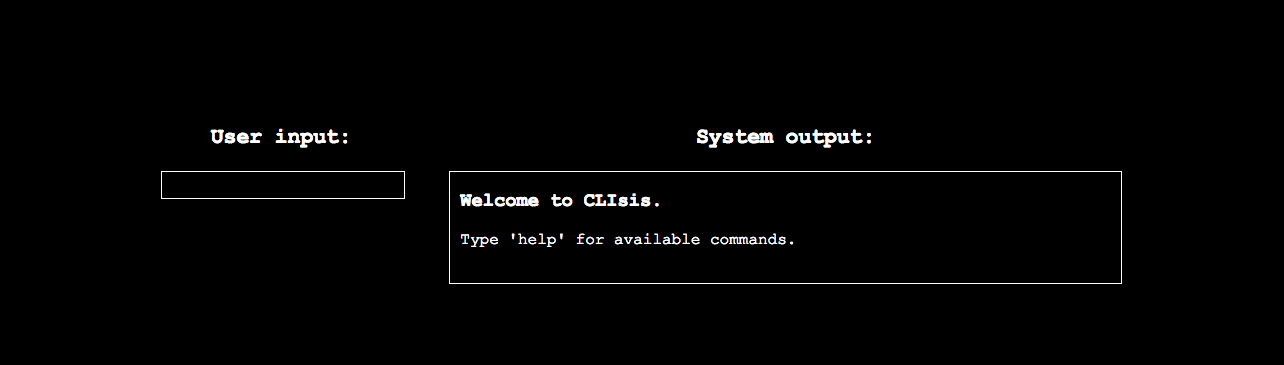
\includegraphics[width=\textwidth]{figures/clisisviews}
	\caption{The start screen of CLIsis}
	\label{figure:clisisviews}
\end{figure}

Furthermore, AngularJS supports filtering variables in views. There are three filters defined in the main module: 
\begin{itemize}
	\item \texttt{substringAfterChar} is used to capture the last part of a string after a certain character.
	\item \texttt{splitToLowerCase} takes a string, splits it on capitalised characters and then joins it with spaces in lower case. This is used so that the speech synthesiser correctly pronounces object keys, which are represented in camel case.
	\item \texttt{startFrom} calculates an index for pagination in displaying a collection.
\end{itemize} 

\subsection{Services}
\label{subsection:services}
Services are processes that are not visible to the user, but serve as a method of sharing code across the application. In most cases their task is related to communication between the front- and back-end of the application.

\begin{itemize}
	\item \bfttt{authentication.js} is used to control the authentication process when logging in. The majority of the code was taken from Incode's Contact app\cite{incod72:online}, with slight alterations where necessary.

	\item \bfttt{services.js} offers a function \texttt{getServices()} to retrieve the available menus from the \acrshort{rest} API.

	\item \bfttt{actions.js} contains several functions: \texttt{getActions()} retrieves all actions for an object or menu, \texttt{invokeAction()} invokes a specific menu action, \texttt{invokeObjectAction()} invokes a specific object action and \texttt{getActionParams()} is a helper function to determine whether the state should be routed to the parameter state or the invocation state.

	\item \bfttt{objects.js} has a function \texttt{getObject()} to retrieve a specific object, \texttt{getCollection()} to get a collection of objects, and two helper functions \texttt{getObjectType()} and \texttt{getObjectId()}, which are used to parse an URL retrieved from the \acrshort{rest} API to determine the object type and id. The function \texttt{buildObjectHref} is used to build the URL that is used in the AngularJS application.

	\item \bfttt{speechService.js} is the service that reads out the user input and system output. It has a method \texttt{speak()} and \texttt{cancelSpeech()}, which are self-explanatory.

	\item Then there are two convenience services: \bfttt{errorService.js} takes care of throwing errors, and \bfttt{rootScopeSanitiser.js} makes sure that the \texttt{\$rootScope}\footnote{The \texttt{\$rootScope} is a global scope accessible by all active controllers. We use it to transfer certain data between controllers.} is not polluted with stale variables.
\end{itemize}

\subsection{Controllers}
\label{subsection:controllers}
Each state of the application has its own controller. The controller ensures that the corresponding view is updated with new information. Aside from their individual behaviour described below, they all make use of AngularJS's \texttt{\$scope.\$watch} functionality, which 'watches' the data in the \texttt{\$scope} for changes. When a change occurs, it triggers the \texttt{speak()} function so the user gets spoken feedback.

\begin{itemize}
	\item \bfttt{InputController.js} is the core controller of our user interface. It is always active and processes the user input that is provided through the input field. Aside from some helper functions that ensure that the focus of the browser is always on the input field and the user can not accidentally tab to the URL bar, the majority of its functionality resides in the function \texttt{evaluateInput()}. This function retrieves the input from the input field, splits it on spaces and then feeds the first element to a switch. The switch recognises 13 different commands. On commands that require one or more parameters, the switch also validates whether they are present and correct.
	\begin{itemize}
		\item \texttt{menus} directs the application to the \texttt{base.home} state.
		\item \texttt{menu} can either take the name of a menu or the index it is displayed with as the parameter. It then directs to the \texttt{base.services} state.
		\item \texttt{actions} broadcasts a \texttt{\$showActions} event. If a menu or object is currently in scope, it shows its actions and they are spoken out.
		\item \texttt{action} can take either the name of an action or the index it is displayed with as the parameter. It then determines whether the action to be invoked has parameters or not; if it does, it directs to the \texttt{base.objectActionParams} or \texttt{base.serviceActionParams} state. If it does not have parameters, it directs to the \texttt{base.objectAction} or \newline \texttt{base.serviceAction} state.
		\item \texttt{field} takes an integer as a parameter to denote which parameter field is to be filled out with the content of the second parameter.
		\item \texttt{submit} confirms that the user has filled out all parameter fields and invokes the action.
		\item \texttt{get} can be used to get an object's property or collection, or an object from a collection. If the parameter is an integer, it directs the application to the desired state. If \texttt{get} is used on a collection, the parameter can also be a string. The controller then filters the contents of the collection with the input, and directs to the \texttt{base.object} state if there is only one result, or to a new \texttt{base.collection} if there are multiple results that fit the parameter.
		\item \texttt{show} without a parameter displays the first five results of a collection. The parameters \texttt{next} and \texttt{previous} turn the pages, with wraparound on the first and last pages.
		\item \texttt{properties} broadcasts a \texttt{\$showProperties} event. If an object is currently in scope, it shows its actions and they are spoken out.
		\item \texttt{collections} broadcasts a \texttt{\$showCollections} event. If an object is currently in scope, it shows its collections and their sizes, and they are spoken out.
		\item \texttt{back} goes back to the previous state. The controller keeps track of a \texttt{previousStates} stack, popping the top state when it goes back.
		\item \texttt{help} lists the help menu.
		\item \texttt{quit} logs the user out of the application and redirects to the login screen.
	\end{itemize}

	\item \bfttt{HomeController.js} gets the menus from the services service and then filters the results based on if there are actions available on each menu. If there are no actions available it is a system menu and bears no functionality for the user.
	
	\item \bfttt{ServiceController.js} gets the menu actions from the actions service.
	
	\item \bfttt{ObjectController.js} gets the object details from the objects service and then parses the results. For all collections that belong to the object, it gets the contents of the collection to display its size in the object view. It also provides a helper method \texttt{typeOf()} that is used in the view.
	
	\item \bfttt{ActionParamController.js} processes the parameters that are required to invoke actions. Parameters can either be simple fields that require a form of text input, or they can be options which are predefined by the system. If the latter is the case, the \acrshort{rest} API exposes them in an extra object key \texttt{choices}. The controller builds the HTML text with these choices. It also listens to a \texttt{\$fieldInputEvent}, which contains the user input to update a parameter field.
	
	\item \bfttt{ActionController.js} calls either \texttt{invokeAction()} or \texttt{invokeObjectAction()}, depending on if the action belongs to a menu or an object. If the action returns one object, the controller routes the application to the object state; if it returns multiple objects, it routes the application to the collection state.
	
	\item \bfttt{CollectionsController.js} gets the collection of objects and manages the pagination in the view. Pagination is essential, as collections can grow large which will cause user frustration if the speech synthesiser speaks the content of a large collection in one go.
	
	\item \bfttt{HelpController.js} sets boolean values based on the state in which the help command was issued, which the view uses to only those commands that are relevant to that state.
	
	\item \bfttt{ErrorController.js} takes care of displaying the correct error message and \bfttt{LoginController.js} handles the login process.
\end{itemize}